\documentclass[11pt]{beamer}
\usetheme{metropolis}

\usepackage[utf8]{inputenc}
\usepackage[spanish]{babel}
\usepackage[T1]{fontenc}

\usepackage{amsmath}
\usepackage{amsfonts}
\usepackage{amssymb}
\usepackage{graphicx}
\usepackage{url}
\usepackage{booktabs}


\DeclareMathOperator{\sen}{sen}
\DeclareMathOperator{\tg}{tg}

\setbeamertemplate{caption}[numbered]


\title[ST: Quechua y Mapudungún]{Low resource speech translation: Quechua y Mapudungún}
\subtitle{Pre-proyecto - NLP}
\author[Barriga, Gazque]{Diego Barriga, Edgar Gazque}
\institute[UNAM]{
    Programa de Posgrado en Ciencia e Ingeniería de la Computación (PCIC)\\
    Universidad Nacional Autónoma de México
}
\date{23 de Marzo 2026}
\titlegraphic{
\includegraphics[width=1cm]{imagens/logo_unam_negro.jpg}}

\setbeamertemplate{navigation symbols}{}


\newcommand{\email}{email}

% TODO: Change to acl style
\bibliographystyle{apalike}

% La agenda se mostrará al inicio de cada sección
\AtBeginSection[]
{
  \begin{frame}
    \frametitle{Table of Contents}
    \tableofcontents[currentsection]
  \end{frame}
}

\begin{document}

\begin{frame}
\titlepage
\end{frame}

\begin{frame}{Contenido}
\tableofcontents
\end{frame}

\section{Especificaciones del reto}

\begin{frame}{Contexto: IWSLT 2026}
\begin{columns}
    \begin{column}{0.6\textwidth}
        \textbf{International Conference on Spoken Language Translation}\footnote{\url{https://iwslt.org/2026/low-resource}}
        \begin{itemize}
            \item Conferencia anual líder en evaluación de sistemas de traducción de habla.
            \item Organiza \textit{Shared Tasks} (tareas compartidas) para benchmark global.
            \item Fomenta la publicación de descripciones de sistemas y hallazgos científicos.
        \end{itemize}
    \end{column}
    \begin{column}{0.4\textwidth}
        \centering
        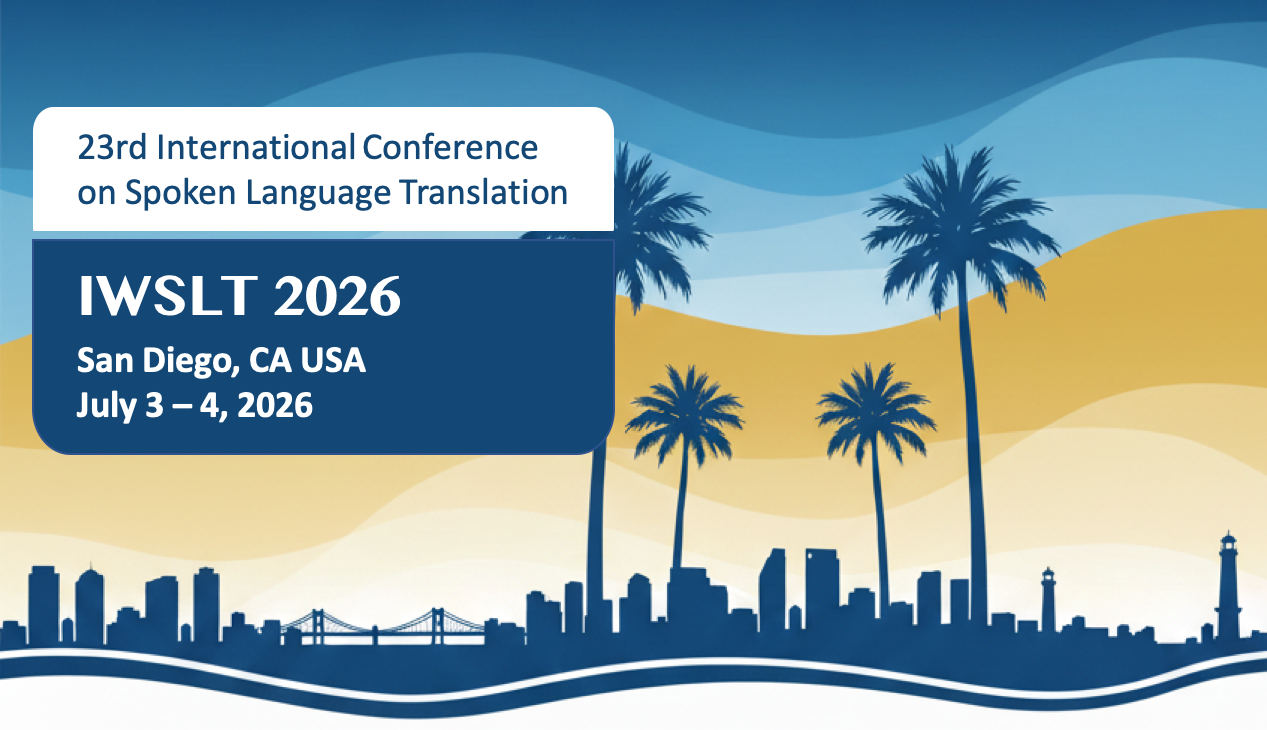
\includegraphics[width=1.0\linewidth]{imagens/iwslt2026_logo.png}
    \end{column}
\end{columns}
\end{frame}

\begin{frame}{Nuestra Participación: \textit{Low-Resource} Track}

    \begin{itemize}
        \item <1-> \textbf{Objetivo General:} El objetivo es evaluar y promover tecnologías de la traducción del habla (\textit{speech translation, ST}) donde los datos son escasos.
        \item <2-> Participaremos en el \textit{shared task} enfocado en lenguas de \textbf{bajos recursos digitales} (\textit{low-resource languages}).
    \end{itemize}
    \vspace{0.5cm}
    \centering
    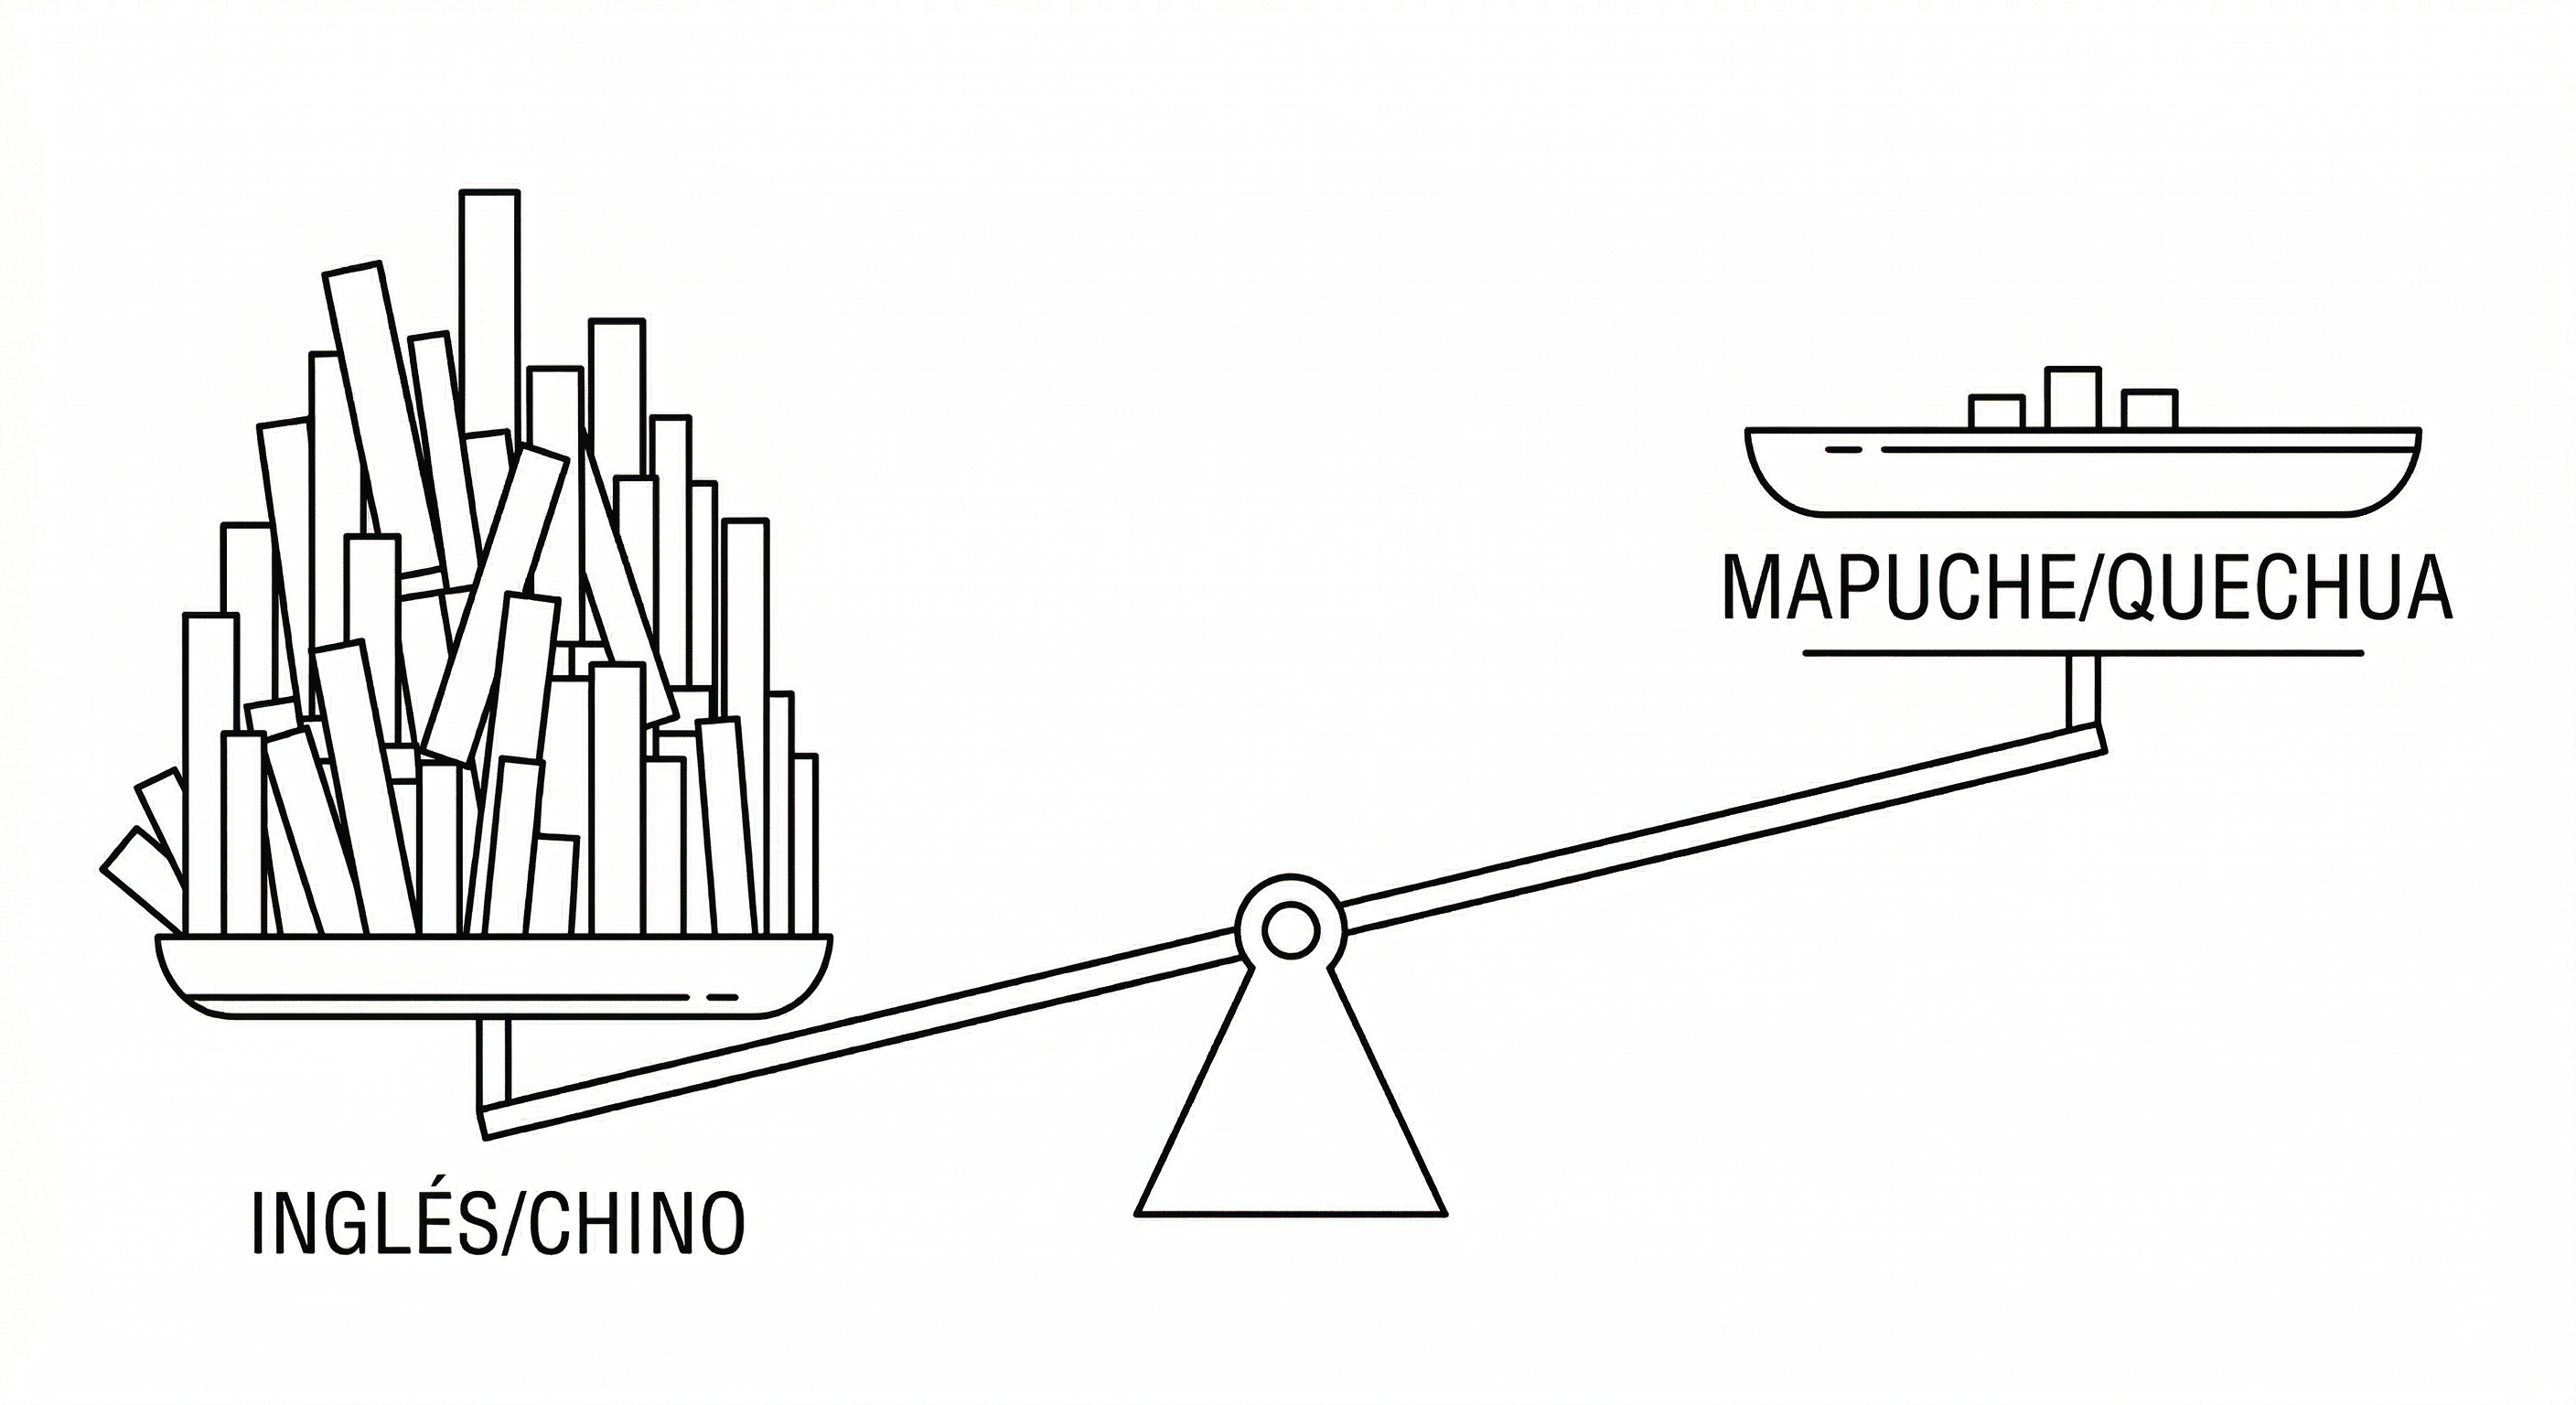
\includegraphics[width=0.7\linewidth]{imagens/balanza.png}
\end{frame}


\begin{frame}{Track 1: Speech to text translation}

\begin{itemize}
    \item <1-> Realizaremos un sistema de \textit{speech translation} para el track 1 el cual contempla 10 lenguas topológicamente diversas.
    \item <2-> Nos enfocaremos en lenguas habladas en América Latina, en partícula, pretendemos hacer un sistema multilingüe Mapuche-Quechua $\rightarrow$ Español.
\end{itemize}

\end{frame}

\begin{frame}{¿Qué es End-to-End Speech Translation?}

    \textbf{Enfoque Clásico (Cascada):}
    \begin{center}
        Audio $\rightarrow$ \fbox{ASR} $\rightarrow$ Texto Transcrito $\rightarrow$ \fbox{MT} $\rightarrow$ Texto Traducido
    \end{center}
    \textit{Problema: Propagación de errores.}

    \vspace{0.5cm}
    \textbf{Enfoque Directo (End-to-End):}
    \begin{center}
        Audio $\rightarrow$ \fbox{\textbf{Modelo Único}} $\rightarrow$ Texto Traducido
    \end{center}
    \textit{Ventaja: Menor latencia, no requiere transcripciones intermedias en entrenamiento.}

\end{frame}


%\begin{frame}{Speech Translation}

%A diferencia de los sistemas de detección automática del habla y traducción habituales, dónde primero se realiza la detección de lo que las personas dicen, se realiza una transcripción en la lengua nativa y después de pasa la transcripción a un modelo de traducción automática, los sistemas de \textit{Speech Translation} realizan el mapeo de voz en lengua nativa a traducción textual en la lengua \textit{target} como un sistema \textit{end-to-end}.

%3\end{frame}

\begin{frame}{Reto principal}

 \large Los modelos estándar de \textit{Deep Learning} requieren miles de horas de audio alineado. Las lenguas originarias \textbf{carecen de estos recursos}.

\end{frame}

\begin{frame}{Preguntas de Investigación (RQs):}

\begin{enumerate}
    \item <1-> \textbf{RQ1:} ¿Es posible \textbf{transferir conocimiento} de modelos masivos pre-entrenados en lenguas mayoritarias hacia lenguas con tipologías drásticamente distintas como el Quechua y Mapuche?
    \item <2-> \textbf{RQ2:} ¿Un enfoque de entrenamiento multilingüe (entrenar ambas lenguas indígenas a la vez hacia el español) mejora el rendimiento individual al \textbf{compartir características} acústicas/semánticas?
    \item <3-> \textbf{RQ3:} ¿Qué técnicas de ajuste eficiente de parámetros (\textit{Adapters}) son más efectivas ante una \textbf{asimetría severa} de datos (90h vs 2h)?
\end{enumerate}

\end{frame}

\begin{frame}{Reto científico}

\begin{itemize}
    \item <1-> Si bien se han mostrado fuertes progresos en el área utilizando \textit{datasets} con recursos abundantes, muchas lenguas del mundo carecen de la cantidad de datos paralelos necesarios para modelos de aprendizaje profundo estándar.
    \item <2-> La comunidad requiere pensar en \textbf{enfoques creativos} para aprovechar los pocos recursos disponibles y, asi, lograr sistemas competitivos y útiles.
\end{itemize}

\end{frame}

\section{Corpus}


\begin{frame}{Características generales}
\textbf{Mapuche (Mapudungún)}
\begin{itemize}
    \item \textbf{Familia:} Araucana.
    \item \textbf{Hablantes:} 100K - 260K \cite{zuniga2006mapudungun}.
    \item \textbf{Países:} Chile, Argentina.
    \item  \textbf{Características:} Lengua no clasificada \cite{zuniga2006mapudungun}.
\end{itemize}

\pause

\textbf{Quechua}
\begin{itemize}
    \item \textbf{Familia:} Araucana.
    \item \textbf{Hablantes:} > 8M
    \item \textbf{Países:} Perú, Ecuador,  Bolivia
    \item \textbf{Característica:} Aglutinante
\end{itemize}
\end{frame}

\begin{frame}{Estadísticas del Dataset (IWSLT proporcionado) I}

	\textbf{Mapudungún (\texttt{arn})} \cite{duan2020resourcecomputationalexperimentsmapudungun}
	\begin{itemize}
		\item \textbf{Region:} Chile
		\item \textbf{Url:} \url{huggingface.co/datasets/mengct00/Mapudungun_iwslt26}
	\end{itemize} \pause

	\textbf{Quechua (\texttt{que})} \cite{cardenas2018siminchik}
	\begin{itemize}
		\item \textbf{Region:} Ayacucho, Peru (Quechua Chanka ISO:quy) y Cusco, Peru (Quechua Collao ISO:quz)
	\item \textbf{Url:} \url{github.com/johneortega/IWSLT2026_Quechua_data}
	\end{itemize}

\end{frame}

\begin{frame}{Estadísticas del Dataset (IWSLT proporcionado) II}

    Se observa un \textbf{severo desbalance} entre las dos lenguas del corpus.

    \vspace{0.3cm}

    \begin{tabular}{lrr}
        \toprule
        \textbf{Métrica} & \textbf{Mapuche} & \textbf{Quechua} \\
        \midrule
        Horas de Audio & \textbf{90} & \textbf{~2} \\
        Frases Alineadas & 42,000 & 698 \\
        Dominio & Narraciones, histórico & Educativo, frases cortas \\
        \bottomrule
    \end{tabular}

\end{frame}

\begin{frame}{Ejemplos}

\begin{block}{Mapuche (Mapudungún)}
    \textit{Kimkevi chi l'awen' pewmamu pu.}
    $\rightarrow$ Conoce el remedio a través de los sueños pues. \\
\end{block}

\pause
\vspace{0.3cm}

\begin{block}{Quechua}
    \textit{chaysi mana ancha qullqinpas kasqachu}. $\rightarrow$ por eso es que no tenia mucho dinero
\end{block}

\end{frame}


\begin{frame}{Características del texto I}
Tamaño promedio de las palabras
\begin{figure}[!tbp]
  \centering
  \begin{minipage}[b]{0.45\textwidth}
    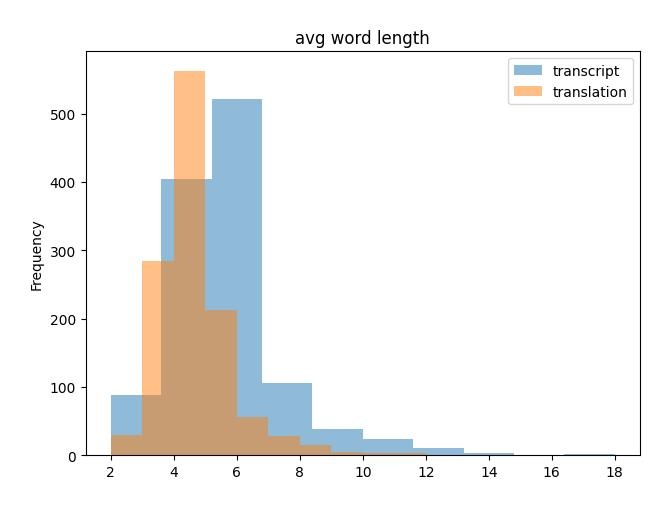
\includegraphics[width=\textwidth]{imagens/Graficas/mapuche/avg_word_length.jpg}
    \caption{Mapuche}
  \end{minipage}
  \hfill
  \begin{minipage}[b]{0.45\textwidth}
    
\includegraphics[width=\textwidth]{imagens/Graficas/quechua/avg_word_length.jpg}
    \caption{Quechua}
  \end{minipage}
\end{figure}
\end{frame}

\begin{frame}{Características del texto II}
Numero de caracteres
\begin{figure}[!tbp]
  \centering
  \begin{minipage}[b]{0.45\textwidth}
    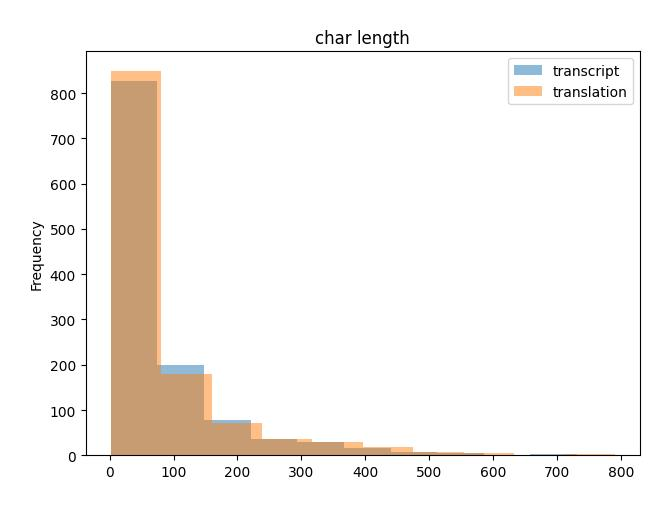
\includegraphics[width=\textwidth]{imagens/Graficas/mapuche/char_length.jpg}
    \caption{Mapuche}
  \end{minipage}
  \hfill
  \begin{minipage}[b]{0.45\textwidth}
    
\includegraphics[width=\textwidth]{imagens/Graficas/quechua/char_length.jpg}
    \caption{Quechua}
  \end{minipage}
\end{figure}
\end{frame}


\begin{frame}{Características del texto III}
Numero de palabras por oracion
\begin{figure}[!tbp]
  \centering
  \begin{minipage}[b]{0.45\textwidth}
    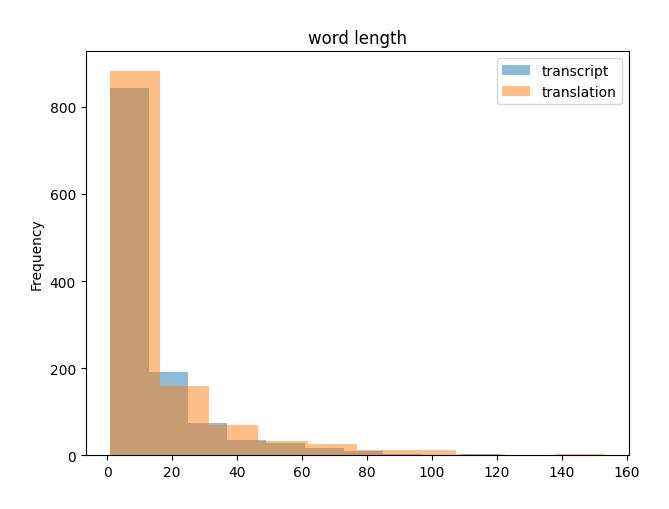
\includegraphics[width=\textwidth]{imagens/Graficas/mapuche/word_length.jpg}
    \caption{Mapuche}
  \end{minipage}
  \hfill
  \begin{minipage}[b]{0.45\textwidth}
    
\includegraphics[width=\textwidth]{imagens/Graficas/quechua/word_length.jpg}
    \caption{Quechua}
  \end{minipage}
\end{figure}
\end{frame}


\section{Propuesta}


\begin{frame}{Modelos preentrenados: Canary}

Canary 1B v2 \cite{koluguri2025granaryspeechrecognitiontranslation}. Un modelo de \textit{1 Billon} de parámetros entrenado con al rededor de 1.7 millones de horas de 25 idiomas. En este trabajo también se entreno con lenguas de bajos recursos como Lituano.

\begin{figure}
  
\includegraphics[width=0.5\linewidth]{imagens/nvidia-logo-horz.png}
\end{figure}
\end{frame}
\begin{frame}{Modelos preentrenados II: SeamlessM4T}
Meta también tiene modelos como SeamlessM4T \cite{seamless2023} con versiones de 1.2 y 2.3 \textit{Billion} parámetros entrenado con 4.5 millones de horas. De igual forma integraron idiomas de bajos recursos en el entrenamiento, como el Uzbeko.
\begin{figure}
  
\includegraphics[width=0.3\linewidth]{imagens/meta_PNG12-1353596828.png}
\end{figure}
En ambos casos los pesos de los modelos están disponibles para uso libre.

\end{frame}

\begin{frame}{Fine-tuning Eficiente (Adapters)}
Dado que tenemos muy pocos datos, un \textit{Full Fine-Tuning} causaría \textbf{overfitting} y es computacionalmente costoso. 
\begin{figure}
  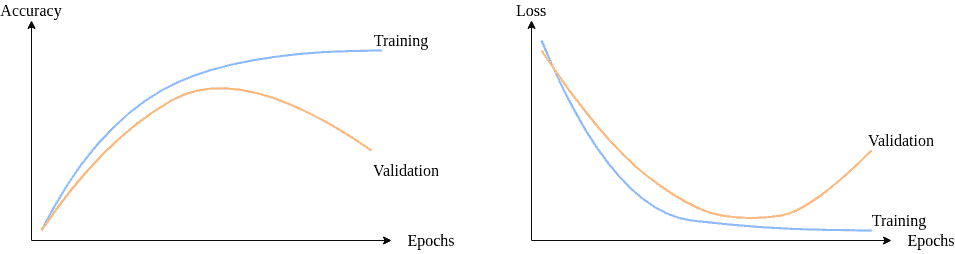
\includegraphics[width=\linewidth]{imagens/overfitting.png}
\end{figure}

Nuestra propuesta: \pause \textbf{Parameter-Efficient Fine-Tuning (PEFT)}

\end{frame}

\begin{frame}{Caracteristicas del adapter \cite{DBLP:journals/corr/abs-2110-04366}}
\begin{itemize}
    \item Funcional: Los parametros entrenables que modificaran el \textit{input}
    \item Inserción: Las salidas del adaptador se integran con la entrada original.
    \item Composición: Cómo se integran las salidas de los adaptadores con las entradas. Ejemplo  una conexión de suma residual o multiplicacion elemento a elemento.
\end{itemize}   
\end{frame}

\begin{frame}{Houlsby Adapter \cite{DBLP:journals/corr/abs-1902-00751}}
    En la implementacion llamado \textit{Linear adapter} 
\begin{figure}
    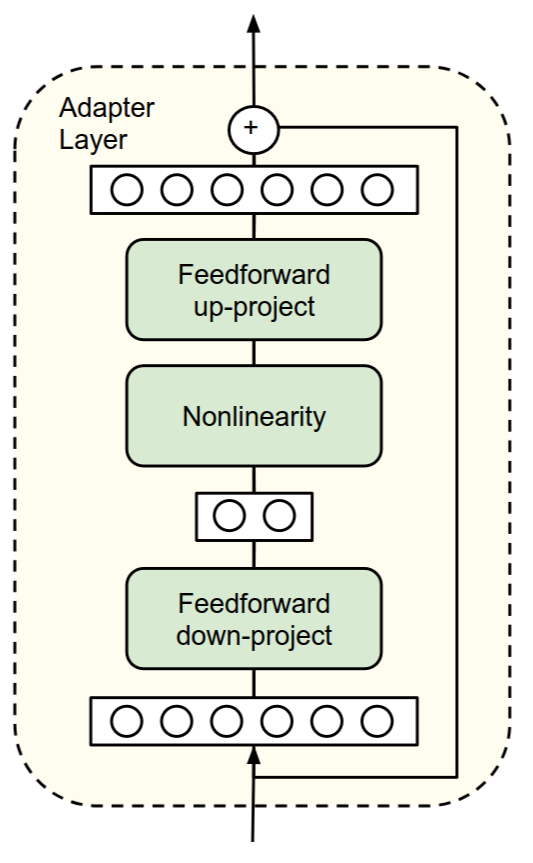
\includegraphics[width=0.3\linewidth]{imagens/Adapter.png}
\end{figure}
Caracteristicas: Modulo Linear Feedforward, LayerNorm, Una sola capa oculta con funcion de activacion.

\end{frame}

\begin{frame}{PEFT}

\begin{itemize}
    \item <1-> Congelamos la mayoría de los pesos del modelo preentrenado (ej. \texttt{canary-1b-v2}).
    \item <2-> Habilitamos pequeñas capas entrenables (\textbf{Adapters}) \cite{houlsby2019parameterefficienttransferlearningnlp}.
    \item <3-> \textbf{Estrategia específica:} Entrenaremos adapters en el \textit{Encoder} para capturar la acústica de las nuevas lenguas.
    \item <4-> Con esta configuracion entrenamos 589,824 parametros de un total de 962,745,344, es decir menor al 0.1 \% 
\end{itemize}

\end{frame}


\section{Registro}

\begin{frame}{Evidencia del registro}

 El registro se llevará a cabo a través de la página de la ACL\footnote{\url{https://2026.aclweb.org/registration/}}. Hasta el momento de esta presentación dicho registro no se ha abierto.

 \begin{figure}
     \centering
     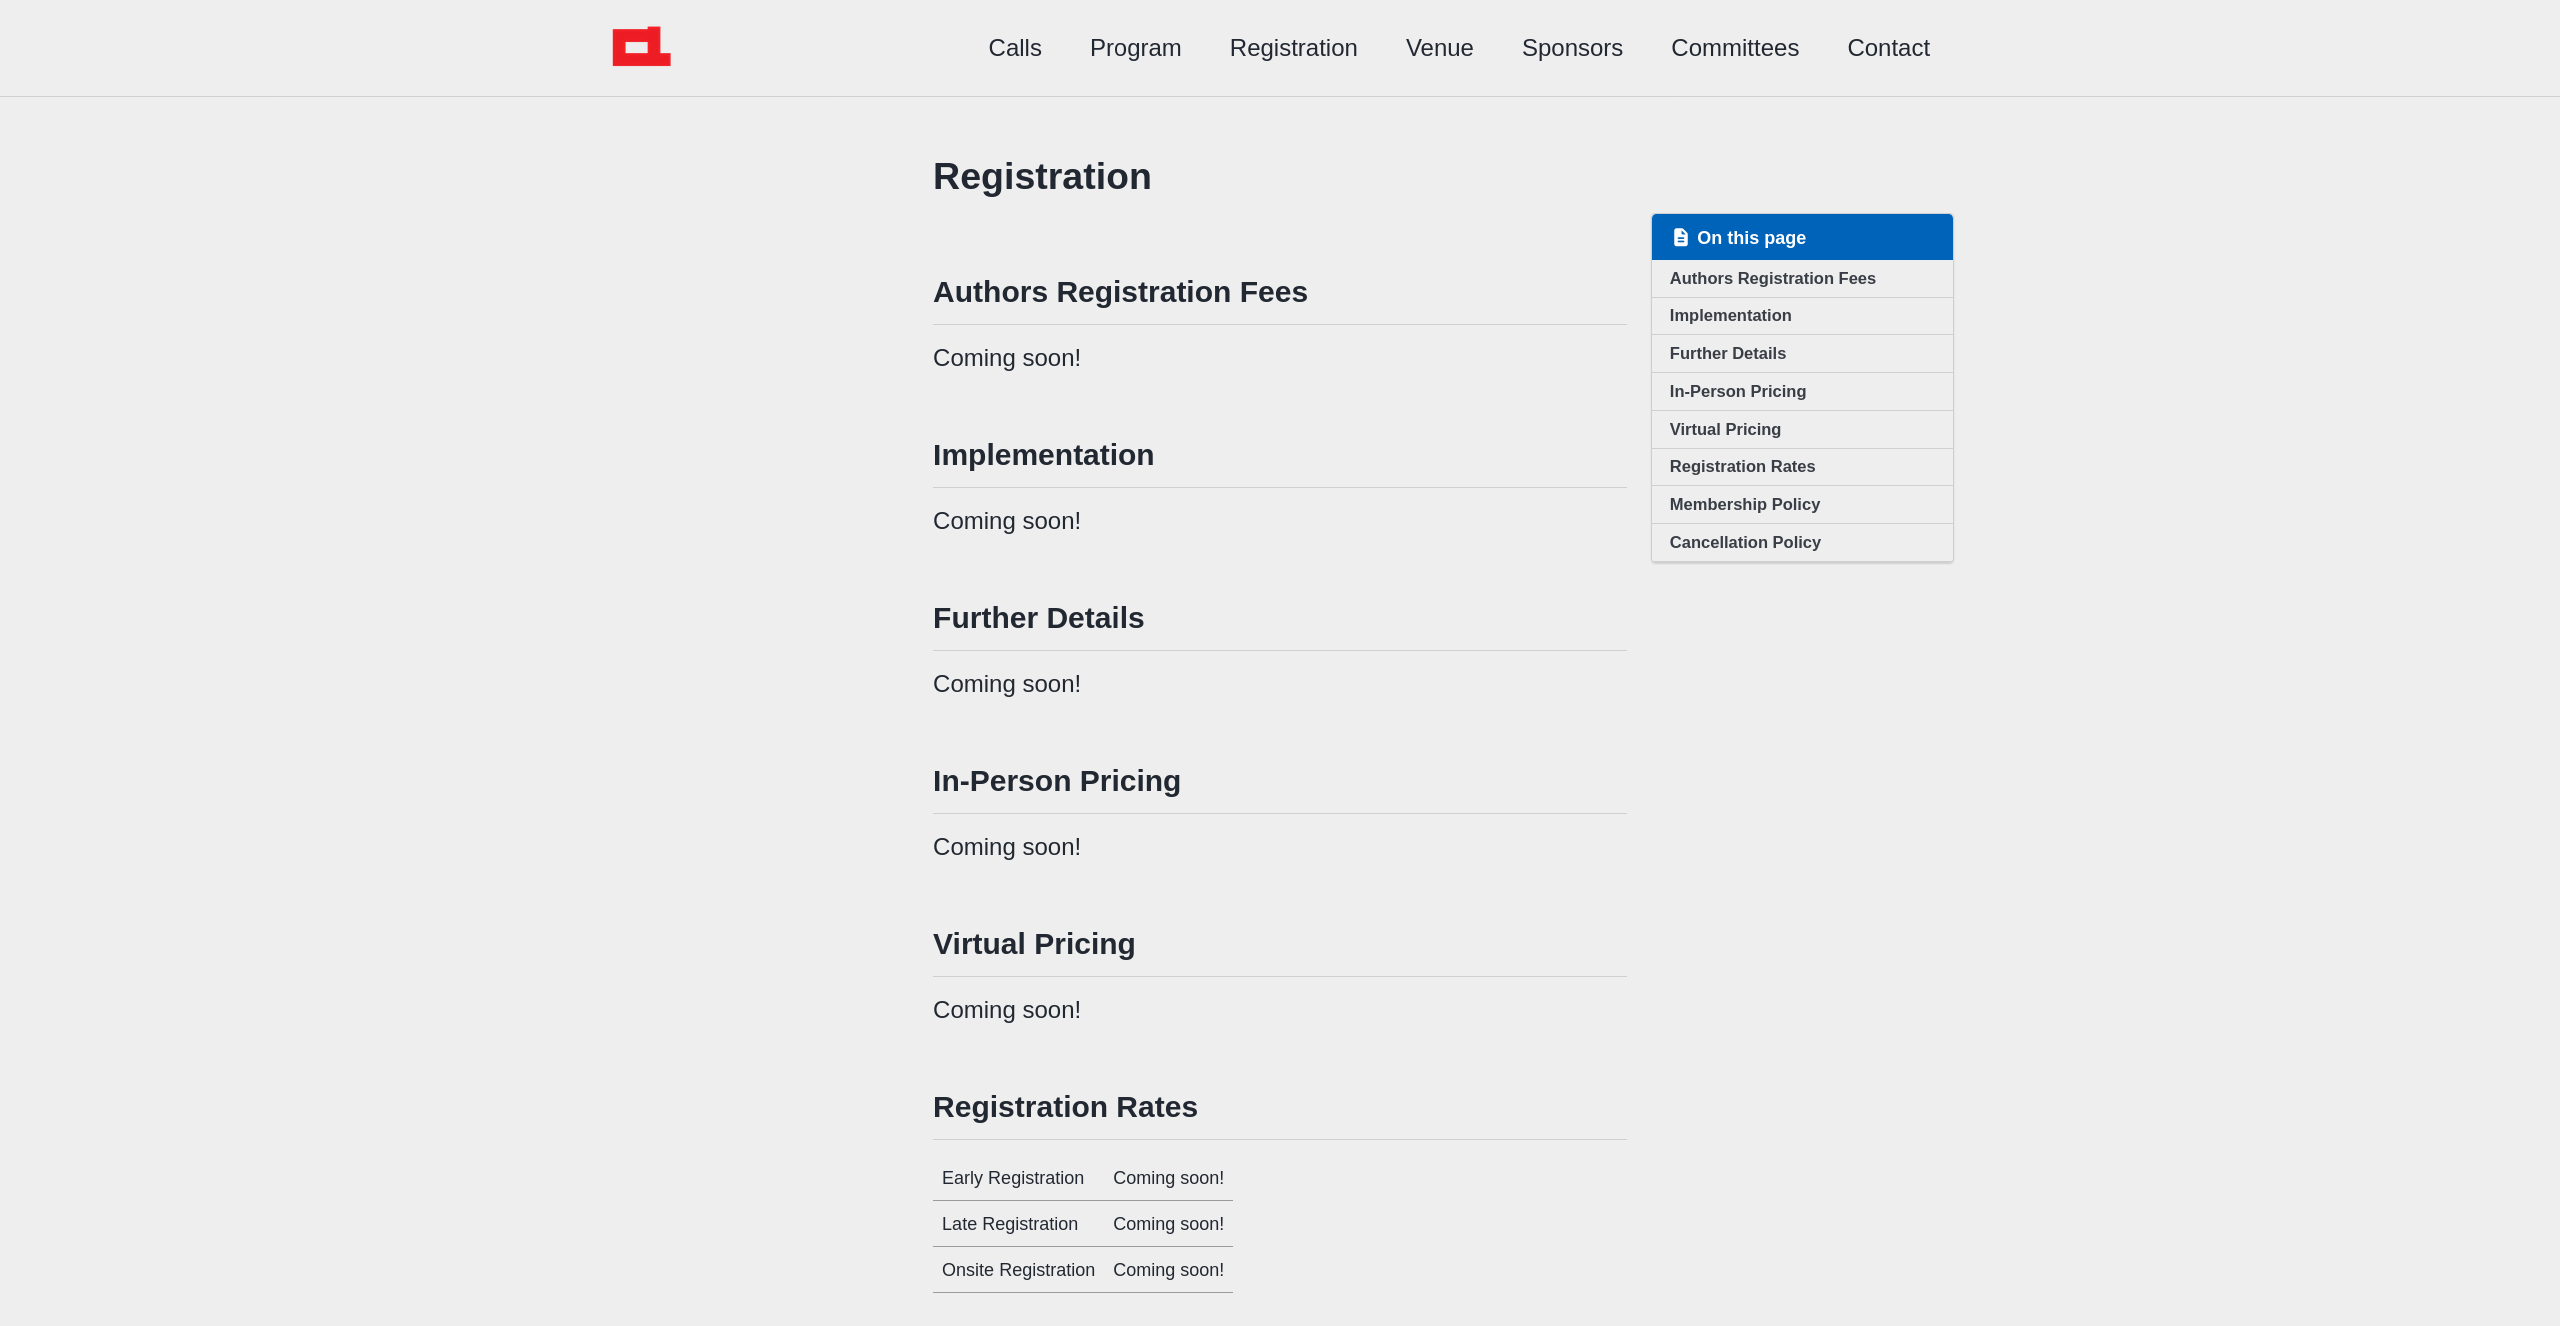
\includegraphics[width=0.8\linewidth]{imagens/registry.png}
 \end{figure}

\end{frame}

\section{Resultados}
\begin{frame}{Primera version}
     \centering
     
\includegraphics[width=0.9\linewidth]{imagens/Resultados/3/training_batch_wer_vs_val_wer.png}
\end{frame}


\begin{frame}{Segunda version I}
     \centering
     
\includegraphics[width=0.9\linewidth]{imagens/Resultados/12/training_batch_wer_vs_val_wer.png}
\end{frame}

\begin{frame}{Segunda version II}
     \centering
     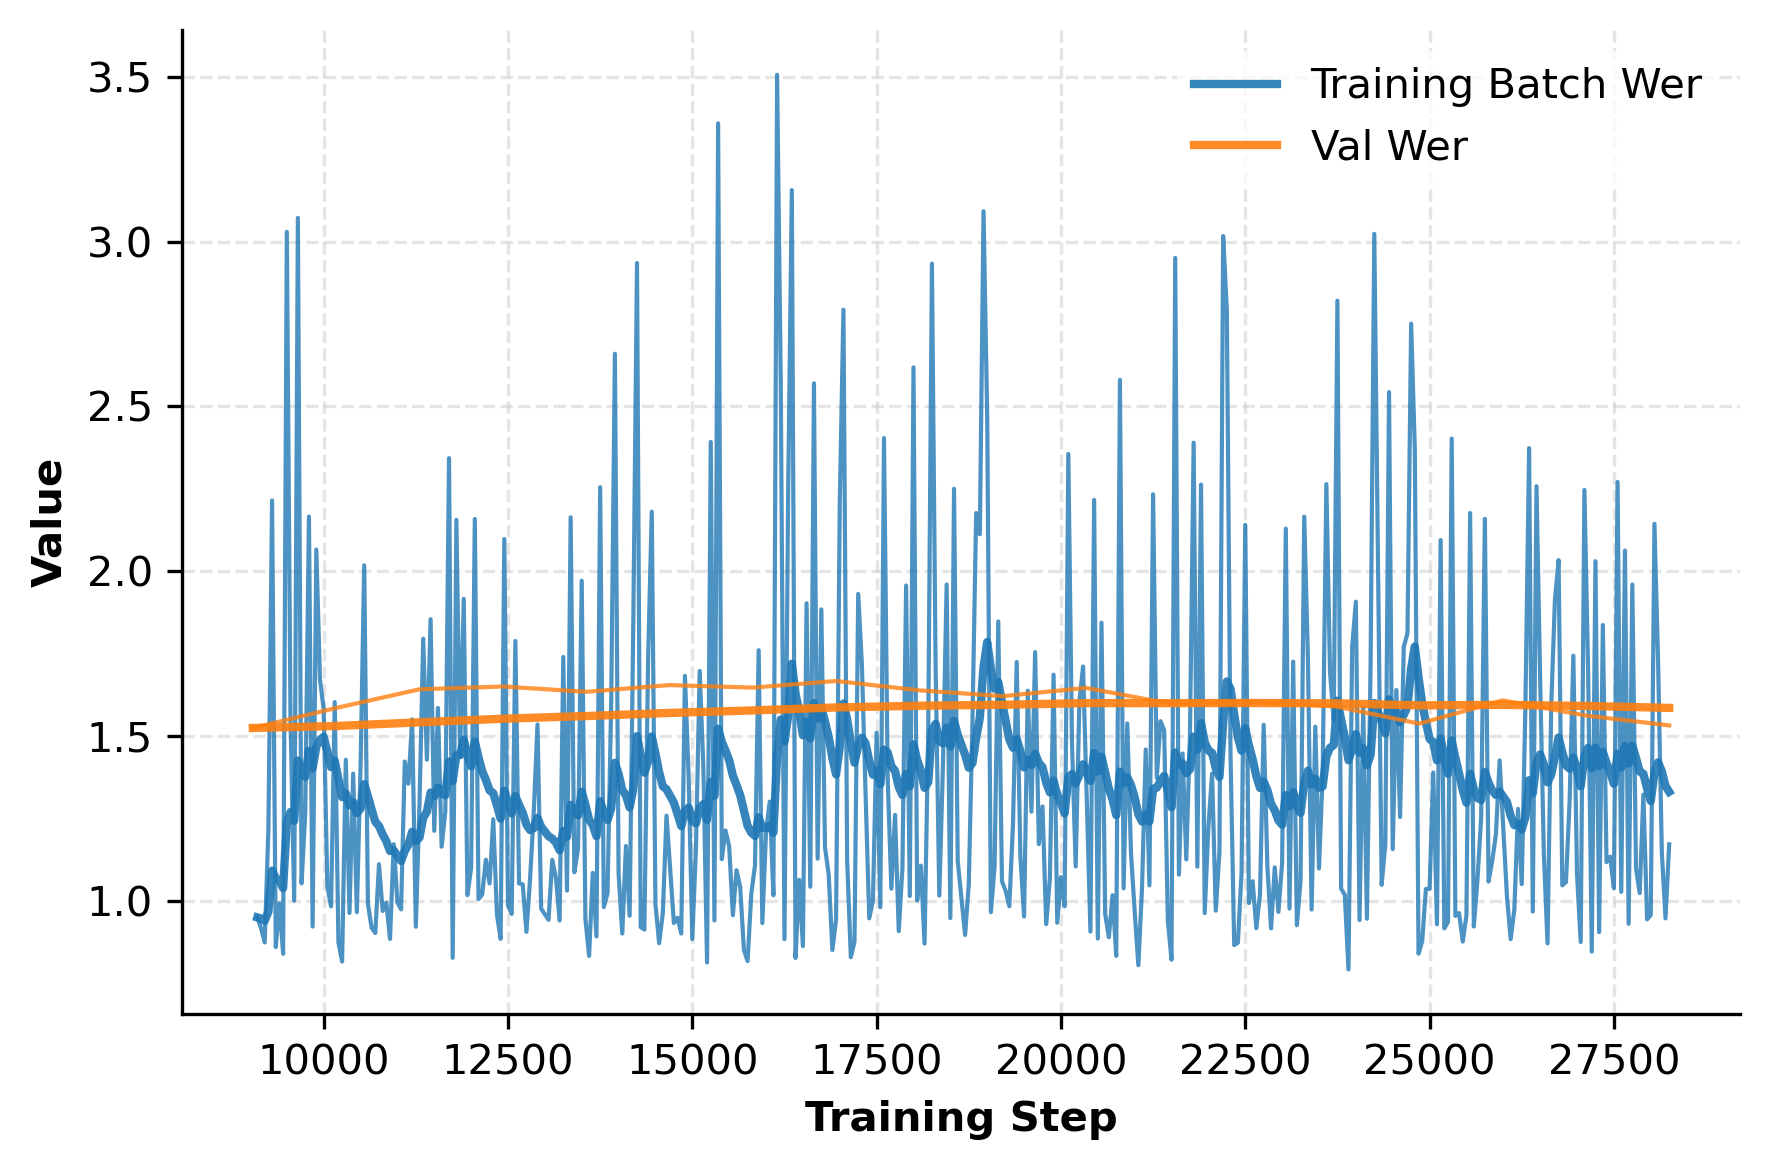
\includegraphics[width=0.9\linewidth]{imagens/Resultados/100/training_batch_wer_vs_val_wer.png}
\end{frame}



\begin{frame}[allowframebreaks]{Referencias}
	\small
    \bibliographystyle{plain}
    \bibliography{referencias}
\end{frame}

\begin{frame}
\centering
\Huge \textbf{¿Preguntas?}

\vspace{1cm}
\normalsize
\textbf{Contacto:} \\
Diego Barriga - \url{dbarriga@ciencias.unam.mx} \\
Edgar Gazque - \url{amilkar@ciencias.unam.mx}
\end{frame}
\end{document}
